\documentclass[../bccalc.tex]{subfiles}
\graphicspath{{\subfix{../figures/}}}
\begin{document}
\chapter{Particle Motion and Integration}
\section{Particle Motion}
\begin{example}
    A particle moves along a horizontal line so that its position at any time $t\geq 0$ is given by \[ s(t)=2t^3-7t^2+4t+5 \] where $s$ is measured in meters and $t$ in seconds.

    (a) Find the velocity at time $t$ and at $t=1$ second.

    $v(t)=s'(t)=6t^2-14t+4$, so $v(1)=-4$ m/s

    (b) When is the particle at rest? Moving left? Moving right? Justify your answers.

    We are looking for $v(t)=0$, $v(t)<0$ and $v(t)>0$.

    We know that $v(t)=0$ at $t=1/3$ and $t=2$.

    It is moving left at $(1/3,2)$ because $v(t)<0$ and right from $(0,1/3)\cup (2,\infty)$ because $v(t)>0$.

    (c) Find the acceleration at time $t$ and at $t=1$ seconds.

    $a(t)=v'(t)=s''(t)=12t-14$, so $a(1)=-2$ m/s$^2$

    (d) Find the displacement of the particle between $t=0$ and $t=3$ seconds. Explain the meaning of your answer.

    $s(3)-s(0)=3$. Displacement was 3 meters to the right.

    (e) Find the distance traveled by the particle between $t=0$ and $t=3$ seconds.

    From $0$ to $1/3$ it travels $0.6296$ meters, from $1/3$ to $2$ it travels an absolute value of $4.6296$ meters, and from $2$ to $3$, it travels $7$ meters, so adding these values gives us $12.2592$ meters.

    (f) When is the particle speeding up? Slowing down? Justify your answer.

    Hint: Since speed is the absolute value of velocity, the particle is 
    \begin{enumerate}
        \item Speeding up when the velocity and acceleration have the same signs.
        \item Slowing down when the velocity and acceleration have opposite signs.
    \end{enumerate}

    Speeding up at $(1/3,7/6)\cup (2,\infty)$ because $v(t)$ and $a(t)$ have the same sign.

    Slowing down $(0,1/3)\cup (7/6,2)$ because $v(t)$ and $a(t)$ have different signs.
\end{example}

\pagebreak
\begin{example}
    A particle moves along a horizontal line so that its position at any time $t\geq 0$ is given by 
    \[ s(t)=t^3-5t^2+2t-3\]
    (a) When is the particle moving right? moving left? Justify your answer.

    This is when $v(t)>0$, or above the $x$-axis for moving right.

    For moving left, it is $v(t)<0$ or below the $x$-axis.

    $v(t)=s'(t)=3t^2-10t+2$.

    Using a calculator, we see that it is moving right from $(0,.2137)\cup (3.11963,\infty)$ because $v(t)>0$.

    It is moving left $(.2137,3.11963)$ because $v(t)<0$.

    (b) Find the distance traveled by the particle from $t=0$ to $t=5$. Justify your answer.

    We have $4$ values of $t$, $0,.2317,3.11963,5$. We can find the $s(t)$ values for all of these and adding up the absolute value of all these gives a value $34.638$.
    
    (c) Find the intervals where the speed is increasing. Justify your answer.

    This is when $v(t)$ and $a(t)$ are the same sign.

    This is in the interval $(.2137,5/3)\cup (3.11963,\infty)$ because $v(t)$ and $a(t)$ have the same sign. 
\end{example}

\ex A particle moves along the $x$-axis so that at any time $t\geq 0$, its velocity is given by $v(t)=3+4.1\cos(0.9t)$. What is the acceleration of the particle at time $t=4$?

\section{Optimization}
\begin{example}
    A swimmer is 2 miles in the ocean and wishes to get to a town 3 miles down the coast which is very rocky.
    The swimmer needs to swim to the shore and then walk along the shore. He can swim at 2 mph and walk at 4 mph. To what point should he swim along the shoreline so that the time it takes to get to town is a minimum?
    \begin{center}
        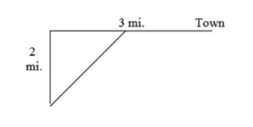
\includegraphics[width=0.3\textwidth]{3.5.1.PNG}
    \end{center}
    We can use the formula $d=rt$ or $t=\frac{d}{r}$ to find this.

    The time is $\frac{\sqrt{x^2+4}}{2}+\frac{3-x}{4}$ and we are trying to find when $T'=0$. The $x$ value that this corresponds to is $x=1.1547$.    
\end{example}

\ex Find the dimensions of a 12-oz. can that can be constructed with the least amount of metal. Justify your answer.

\section{Antiderivatives and Indefinite Integrals}
If you were given $f'(x)=3x^2$ and asked what function $f(x)$ had this derivative, what would you say?

You would say $f(x)=x^3$ or $f(x)=x^3-7$ or any other constant.

$f(x)$ is called the antiderivative of $f'(x)$.

The symbol $\int g(x)$ is the indefinite integral. The term indefinite integral is a synonym for antiderivative.

We can get formulas for antiderivatives by reversing the differentiation rules.

Integration Rules:
\begin{itemize}
    \item $\int x^n dx = \frac{x^{n+1}}{n+1}+C, n\neq -1$
    \item $\int \cos u du=\sin u+C$
    \item $\int \sin u du=-\cos u+C$
    \item $\int \sec^2 u du = \tan u +C$
    \item $\int \csc^2 u du = -\cot u +C$
    \item $\int \sec u \tan u du = \sec u +C$
    \item $\int \csc u \cot u du = -\csc u +C$
\end{itemize}

Properties of Indefinite Integrals:
\begin{itemize}
    \item $\int (f(x)\pm g(x))dx = \int f(x)dx \pm \int g(x)dx$
    \item $\int kf(x)=k\int f(x)dx$, where $k$ is a constant 
\end{itemize}
Note that $\int f(x)\cdot g(x)dx\neq \int f(x)dx\cdot \int g(x)dx$ and $\int \frac{f(x)}{g(x)}\neq \frac{\int f(x)dx}{\int g(x)dx}$

\begin{example}
    \[ \int (3x^2-5x+4)dx =\]

    Use the integration rules to get $\frac{3x^3}{3}-\frac{5x^2}{2}+4x+C$ or $x^3-\frac{5}{2}x^2+4x+C$.
\end{example}

There isn't a product rule of a quotient rule for antiderivatives so you must simplify first.
\begin{example}
    \[ \int (2x-1)(x+3)dx = \]
    Simplifying gives $\int 2x^2+6x-x-3 dx = \int 2x^2+5x-3dx$.

    This is equal to $\frac{2x^3}{3}+\frac{5x^2}{2}-3x+C$.
\end{example}

\ex $\int \frac{x^2-2x+7}{\sqrt{x}}dx =$

\begin{example}
    Solve the differential equation $f'(x)=6x^2, f(1)=-3$.

    When we integrate we get $f(x)=\frac{6x^3}{3}+C$.

    $f(x)=2x^3+C$, and we have the condition $f(1)=-3$. so we can plug this in to get $-3=2(1)^3+C$ which gives $C=-5$.

    Therefore $f(x)=2x^3-5$.
\end{example}

\ex Solve the differential equation $f''(x)=\cos x, f'(0)=3, f(0)=-2$.

\ex A particle moves along the $x$-axis at a velocity of $v(t)=4t^3-3t^2+5, t\geq 0$. At time $t=2$, its position is $x=3$. Find the acceleration function and find the position function.
\section{Integration using U-Substitution}
When we differentiated composite functions, we used the Chain Rule. The reverse process is called u-substitution.

\begin{example}
    \[ \int (x^2+1)^5(2x)dx=\]
    If we let $u=x^2+1$, we can see that $\frac{du}{dx}=2x$ which implies that $du=2xdx$.

    We can rewrite this function now as $\int u^5 du = \frac{u^6}{6}+C$.

    Therefore, the integral comes out to $\frac{(x^2+1)^6}{6}+C$.
\end{example}

\ex $\int x^2(2x^3+5)^4 dx=$

\begin{example}
    \[ \int x\sqrt{x^2+3}dx = \]
    We let $u=x^2+3$ and $\frac{du}{dx}=2x$. This gives $\frac{1}{2}du = xdx$.

    So we can write the integral as $\frac{1}{2}\int u^{1/2}du = \frac{1}{2}\cdot \frac{2}{3}u^{3/2}+C$.

    The result is $\frac{1}{3}(x^2+3)^{3/2}+C$.
\end{example}

\ex $\int \frac{x}{\sqrt{3x^2+4}}dx=$

\ex $\int \cos(3x)dx=$

\ex Solve the differential equation $\frac{dy}{dx}=\frac{9x^2}{\sqrt{1+x^3}}+5x$

\section{Integration and Area Under a Curve}
\begin{example}
    A car is traveling so that its speed is never decreasing during a 12-second interval. The speed at various moments in time is listed in the table below.
    \begin{center}
        \begin{tabular}{|c|c|c|c|c|c|}
        \hline 
        Time in Seconds & 0 & 3 & 6 & 9 & 12\\
        \hline 
        Speed in ft/sec & 30 & 37 & 45 & 54 & 65\\
        \hline
    \end{tabular}
    \end{center}

    (a) Estimate the distance traveled by the car during the 12 seconds by finding the areas of four rectangles drawn at the heights of the left endpoints. This is called a left Riemann sum.

    If you draw a rough sketch of the graph and use the rectangle heights, you can get four rectangles and find the areas.

    You should get $3(30)+3(37)+3(45)+3(54)$

    (b) Estimate the distance traveled by the car during the 12 seconds by finding the areas of four rectangles drawn at the heights of the right endpoints. This is called a right Riemann sum.

    Similar process: $3(37)+3(45)+3(54)+3(65)$

    (c) Estimate the distance traveled by the car during the 12 seconds by finding the areas of two rectangles drawn at the heights of the midpoints. This is called a midpoint Riemann sum.

    You get $6(37)+6(54)$.
\end{example}

\ex Given the function $y=x^2+1$, estimate the area bounded by the graph of the curve and the $x$-axis on $[0,2]$ by using:

(a) a left Riemann sum with $n=4$ equal subintervals.

(b) a right Riemann sum with $n=4$ equal subintervals

(c) a midpoint Riemann sum with $n=4$ equal subintervals

\section{Riemann Sums and the Definite Integral}
To estimate the area bounded by the graph of $f(x)$ and the $x$-axis between the vertical lines $x=a$ and $x=b$, partition the area and divide it into subintervals.
We previously drew rectangles with the height at the left endpoint or the right endpoint or at the midpoint of the interval. For this, we will draw rectangles at some general point within the subinterval, not necessarily at the left endpoint or the right endpoint or at the midpoint of the interval.

Let $x=c_k$ be any point in the $k$th subinterval. Draw a rectangle with a height of $f(c_k)$.

The area of this rectangle is $f(c_k)\Delta x$.

The sum of all the rectangles is $\sum_{k=1}^n f(c_k)(\Delta x_k)$.

This sum is called a Riemann sum.

To find the exact area under the curve we use 
\[ \lim_{n\to \infty} \sum_{k=1}^n f(c_k)(\Delta x_k) \]

\begin{definition}[Definite Integral]
    Defines as 
    \[ \int_a^b f(x)dx = \lim_{n\to \infty}\sum_{k=1}^n (f(c_k))(\Delta x_k) \]
    or 
    \[ \int_a^b f(x)dx=\lim_{\Delta x_k \to 0}\sum_{k=1}^n (f(c_k))(\Delta x_k) \]
\end{definition}

The area bounded by $y=f(x)$ and the $x$-axis on $[a,b]=\int_a^b f(x)dx$.

Properties of Definite Integrals 
\begin{itemize}
    \item $\int_a^a f(x)dx=0$
    \item $\int_b^a f(x)dx=-\int_a^b f(x)dx$
    \item $\int_a^b k\cdot f(x)dx=k\int_a^b f(x)dx$
    \item If $c$ lies between $a$ and $b$, then $\int_a^b f(x)dx=\int_a^c f(x)dx+\int_c^b f(x)dx$
    \item $\int_a^b (f(x)+g(x))dx=\int_a^b f(x)dx+\int_a^b g(x)dx$
    \item $\int_a^b (f(x)-g(x))dx=\int_a^b f(x)dx-\int_a^b g(x)dx$
\end{itemize}

Note: $\int_a^b (f(x)\cdot g(x))dx\neq \int_a^b f(x)dx\cdot \int_a^b g(x)dx$ and $\int_a^b \left(\frac{f(x)}{g(x)}\right)dx\neq \frac{\int_a^b f(x)dx}{\int_a^b g(x)dx}$
\pagebreak
\begin{example}
    Evaluate by using a geometric formula.
    \[ \int_1^6 4 dx \]
    If we draw a rectangle of this, we get the area of the rectangle as 20.
\end{example}

\begin{example}
    Evaluate by using a geometric formula.
    \[ \int_1^3 (x+2)dx \]
    This is a triangle, the area is 8.
\end{example}

\ex $\int_{-2}^2 \sqrt{4-x^2}dx = $

\ex $\int_{-4}^4 f(x)dx = $

\begin{example}
    Given $\int_0^3 f(x)dx=4$ and $\int_3^7 f(x)dx=-$. Find:

    (a) $\int_0^7 f(x)dx$

    Answer is 3.

    (b) $\int_3^7 2f(x)dx$ 

    This is $2\int_3^7 f(x)dx = -2$

    (c) $\int_5^5 f(x)dx=$.

    0
\end{example}

\section{Fundamental Theorem of Calculus}
\begin{theorem}[Fundamental Theorem of Calculus]
    \[ \int_a^b f'(x)dx= [f(x)]^{x=b}_{x=a}=f(b)-f(a) \]
\end{theorem}

\begin{example}
    \[ \int_1^2 (x^2+3)dx = \]

    We are just doing 
    \[ \left[ \frac{x^3}{3}+3x\right]^2_1 = \left(\frac{8}{3}+6\right)-\left(\frac{1}{3}+3\right) = \frac{16}{3}\]
\end{example}

\ex $\int_1^9 \frac{x-4}{\sqrt{x}}dx=$

\ex $\int_0^{\pi/4}\sec^2 xdx=$

\ex $\int_0^3 |2x-1|dx =$.
Note, $|a|=\begin{cases}
    a \text{ if } a\geq 0 \\
    -a \text{ if }a<0
\end{cases}$

\begin{example}
    Find the area bounded by the graph of $y=2x^2-3x+2$, the $x$-axis, and the vertical lines $x=0$ and $x=2$.

    The integral is $\int_0^2 2x^2-3x+2dx$.

    If we integrate this and use the bounds, we get the answer of $\left(\frac{16}{3}-\frac{12}{2}+4\right)-(0)$.
\end{example}
\pagebreak
\section{U-Substitution with Definite Integrals}
\begin{example}
    \[ \int_1^2 x(x^2+1)^3 dx = \]

    We let $u=x^2+1$, and $\frac{du}{dx}=2x$.

    We also have $\frac{1}{2}du=xdx$.

    When $x=1$ then $u=2$ and when $x=2$ then $u=5$.

    So we know integrate $\frac{1}{2}\int_2^5 u^3 du$ to get the result $\frac{1}{2}\left[\frac{5^4}{4}-\frac{2^4}{4}\right]$.
\end{example}

\ex $\int_0^2 \frac{x}{\sqrt{1+2x^2}}dx=$

\ex $\int_{\pi/12}^{\pi/9}\sin(3x)dx=$

\ex Find the area bounded by the graph of $y=x\sqrt{x^2+1}$ and the $x$-axis on the interval $[0,2]$.

\begin{example}
    Water is being pumped into a tank at a rate given by $R(t)$. A table of values of $R(t)$ is given.
    \begin{tabular}{|c|c|c|c|c|c|}
        \hline
        $t$ (min.) & 0 & 5 & 9 & 15 & 20\\ \hline 
        $R(t)$ (gal/min) & 14 & 18 & 20 & 27 & 32\\ \hline
    \end{tabular}

    (a) Use the data from the table and four subintervals to find a left Riemann sum to approximate $\int_0^{20}R(t)dt$.

    \[ 14(5)+18(4)+20(6)+27(5) \]

    (b) Use data from the table and four subintervals to find a right Riemann sum to approximate $\int_0^{20}R(t)dt$.

    \[ 18(5)+20(4)+27(6)+32(5) \]
\end{example}

\section{Another Kind of U-Substitution}
Sometimes the u-substitution method we have learned does not work, and we need to do something different to integrate.

\begin{example}
    \[ \int x\sqrt{2x-1}dx = \]

    We can let $u=2x-1$ and $\frac{du}{dx}=2$. We also see that $\frac{u+1}{2}=x$.

    So we can write the integral as $\frac{1}{2}\int \frac{u+1}{2}\cdot u^{1/2}$.

    The result is $\frac{1}{4}\left(\frac{2}{5}u^{5/2}+\frac{2}{3}u^{3/2}\right)+C$.
\end{example}

\ex $\int_1^5 \frac{x}{\sqrt{2x-1}}dx=$

\ex $\int_0^7 \frac{x}{\sqrt[3]{x+1}}dx=$

If a function $f$ is even, then $f$ has $y$-axis symmetry so $\int_{-a}^a f(x)dx=2\int_0^a f(x)dx$.

If a function $f$ is odd, then $f$ has origin symmetry so $\int_{-a}^a f(x)dx=0$.

\begin{example}
    Given $f(x)$ is even and $\int_0^5 f(x)dx=3$. Find:

    (a) $\int_{-5}^5 f(x)dx$

    $2(3)=6$

    (b) $\int_{-5}^0 f(x)dx$

    3

    (c) $\int_{-5}^5 4f(x)dx$

    $4(6)=24$.
\end{example}

\ex Given $f(x)$ is odd and $\int_0^5 f(x)dx=3$. Find:

(a) $\int_{-5}^5 f(x)dx$

(b) $\int_{-5}^0 f(x)dx$

(c)$ \int_{-5}^5 4f(x)dx$

\section{Fundamental Theorem of Calculus}
\begin{example}
    Given $\frac{dy}{dx}=3x^2+4x-5$ with the initial condition $y(2)=-1$. Find $y(3)$.

    Method 1: Integrate $y=\int(3x^2+4x-5)dx$ and use the initial condition to find $C$. Then write the particular solution, and use your particular solution to find $y(3)$.

    $y=x^3+2x^2-5x+C$. Plugging in the initial conditions gives $C=-7$.

    Therefore $y=x^3+2x^2-5x-7$, so $y(3)=23$.

    Method 2: Use the Fundamental Theorem of Calculus: $\int_a^b f'(X)dx=f(b)-f(a)$

    This gives $\int_2^3 f'(x)dx=f(3)-f(2)\implies f(3)=-1+\int_2^3 f'(x)dx$.

    So $=1+[x^3+2x^2-5x]_2^3 = f(3)=23$.
\end{example}

Sometimes there is no antiderivative, so you must use Method 2 and a graphing calculator.

\begin{example}
    $f'(x)=\sin(x^2)$ and $f(1)=-5$. Find $f(2)$.

    $\int_1^2 \sin(x^2)dx=f(2)-f(1)$.

    $f(2)=-5+\int_1^2 \sin(x^2)dx = -4.50549$.
\end{example}
\pagebreak
\begin{example}
    \begin{center}
        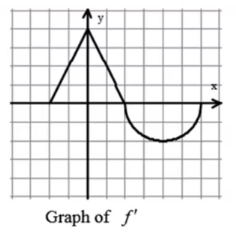
\includegraphics[width=0.3\textwidth]{4.1.1.PNG}
    \end{center}
    The graph of $f'$ consists of two line segments and a semicircle as shown above. Given that $f(-2)=5$, find 

    (a) $f(0)$

    We are finding $\int_{-2}^0 f'(x)dx=f(0)-f(-2)$. So $f(0)=5+\int_{-2}^0 f'(x)dx = 9$.

    (b) $f(2)$

    $f(2)=5+\int_{-2}^2 f'(x)dx=13$.

    (c) $f(6)$

    $f(6)=5+\int_{-2}^6 f'(x)dx=13-2\pi$.
\end{example}

\ex The graph of $f'$ is shown. Use the figure and the fact that $f(3)=5$ to find 
\begin{center}
    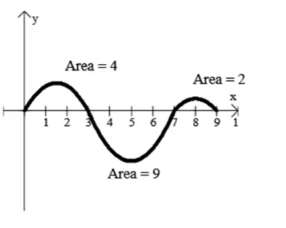
\includegraphics[width=0.3\textwidth]{4.1.2.png}
\end{center}
(a) $f(0)$

(b) $f(7)$

(c) $f(9)$

\ex A pizza with a temperature of $95^{\circ}$C is put into a $25^{\circ}$C room when $t=0$. The pizza's temperature is decreasing at a rate of $r(t)=6e^{-0.1t\circ}$C per minute. Estimate the pizza's temperature when $t=5$ minutes.

\begin{example}
    If $f(3)=5$, $f'$ is continuous, and $\int_3^8 f'(x)dx=20$, find the value of $f(8)$.

    $\int_3^8 f'(x)dx=f(8)-f(3)$. We know $20=f(8)-5$, so $f(8)=25$.
\end{example}

\ex If $\int_{-1}^4 (3f(x)+2)dx=28$, find $\int_{-1}^4 f(x)dx$.

\ex $f(x)=\begin{cases}
    3x-1, x\leq 2\\
    x^2+1, x>2
\end{cases}$.

Evaluate $\int_{-1}^4 f(x)dx$.

\section{Average Value of a Continuous Function}
\begin{theorem}[Mean Value Theorem for Integrals]
    If $f$ is continuous on $[a,b]$, then there exists a number $c$ in $[a,b]$ such that $\int_a^b f(x)dx=f(c)(b-a)$.
\end{theorem}

The geometric interpretation of the Mean Value Theorem for Integrals is that, for a positive function $f$, there is a number $c$ between $a$ and $b$ such that the rectangle with base $[a,b]$ and height 
$f(c)$ has the same area as the region under the graph of $f$ from $a$ to $b$. In other words, $c$ is the value of $x$ on $[a,b]$ where you can build a ``perfect'' rectangle - a rectangle whose area is exactly equal to the area of the region under the graph of $f$ from $a$ to $b$.

The value $f(c)$ is called the average value of the function $f$ and is defined by:
\[ f_{ave}=\frac{1}{b-a}\int_a^b f(x)dx\]

\begin{example}
    Given $f(x)=1+x^2$ and the interval $[-1,2]$.

    (a) Find the average value of $f$ on the given interval.

    $f_{ave}=\frac{1}{3}\int_{-1}^2 1+x^2dx = 2$.

    (b) Find $c$ such that $f_{ave}=f(c)$.

    $2=1+c^2$ implies $c=1$.
\end{example}

\begin{example}
    The table below gives values of a continuous function $f$. Use a left Riemann sum with three subintervals and values from the table to estimate the average value of $f$ on $[5,17]$.
   \[ \begin{tabular}{|c|c|c|c|c|}
        \hline 
        x & 5 & 9 & 12 & 17\\ \hline 
        f(x) & 23 & 29 & 36 & 27\\\hline
        
    \end{tabular}\]

    This is $\frac{1}{17-5}\int_5^{17}f(x)dx=\frac{1}{12}[4(23)+3(29)+5(36)]=29.9167$
\end{example}

\ex A study suggests that between the hours of 1:00 PM and 4:00 PM on a normal weekday, the speed of the traffic on a certain freeway exit is modeled by the formula $S(t)=2t^3-21t^2+60t+20$ where the speed is 
measured in kilometers per hour and $t$ is the number of hours past noon. Compute the average speed of the traffic between the hours of 1:00 PM and 4:00 PM.

\pagebreak
\ex Suppose that during a typical winter day in Minneapolis, the temperature (in degrees Celsius) $x$ hours after midnight is shown in the figure below.
\begin{center}
    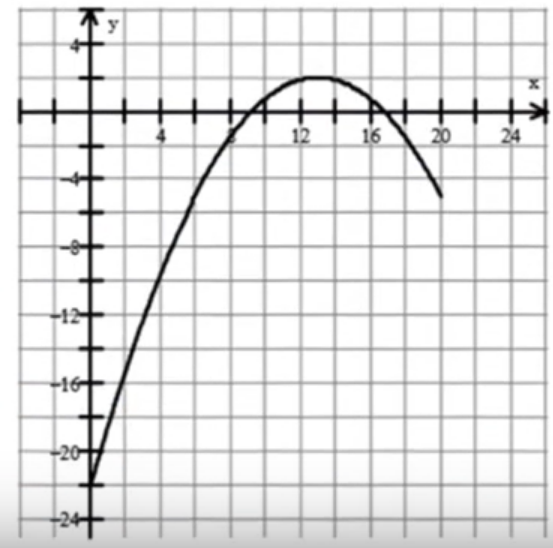
\includegraphics[width=0.3\textwidth]{4.2.1.png}
\end{center}
(a) Use a midpoint Riemann sum with four equal subintervals to approximate the average temperature over the time period from 4:00 AM to 8 PM.

(b) Use your answer from part (a) to estimate the time when the average temperature occurred.

\ex Find the average value of the function on the given interval without integrating.
\[ f(x)=\begin{cases}
    3-x \text{ if } -1\leq x\leq 3 \\
    2x-6 \text{ if } 3<x\leq 6
\end{cases} \] on $[-1,6]$


\end{document}